\documentclass[11pt,pdftex,portrait,letterpaper]{article}
\usepackage[hdivide={1in,*,1in},
            vdivide={1in,*,1in},
%            showframe
            ]{geometry}

\usepackage{graphicx}
\usepackage{longtable}
\usepackage{acronym}
\usepackage{verbatim}
\usepackage{subfigure}
\usepackage{fancyhdr}
\pagestyle{fancy}
\usepackage{listings}
\usepackage{color}
\usepackage{lastpage}

% Default margins are too wide all the way around. Reset them here
\setlength{\topmargin}{-.5in}
\setlength{\textheight}{9in}
\setlength{\oddsidemargin}{.125in}
\setlength{\textwidth}{6.25in}

\lhead{ECEN 898}
\chead{}
\rhead{\thepage\ of \pageref{LastPage}}
%\lfoot{\hline}
\lfoot{}
\cfoot{\small{University of Nebraska - Lincoln Department of Electrical Engineering}}
\rfoot{}
\renewcommand{\footrulewidth}{0.5pt}


% Modify parameters of Listings
\lstset{ 
language=C,
basicstyle=\scriptsize,
numbers=left,
numberstyle=\footnotesize,
stepnumber=1,
numbersep=10pt,
backgroundcolor=\color{white},
frame=single,
captionpos=b,
breaklines=true,
breakatwhitespace=false
}

\begin{document}

\vspace*{30ex}
\begin{center}

\textbf{Project 04 - BIOS Multithread }\\

\vspace{4ex}
Introduction to Embedded Systems - University of Nebraska \\

\vspace{4ex}
Zach Swanson\\

\end{center}


\pagebreak
\tableofcontents
%\pagebreak
%\listoffigures
%\addcontentsline{toc}{section}{{\bf List of Figures}}
\pagebreak


\section{Introduction}

The purpose of this project was to introduce tasks (TSK), an additional type of BIOS thread not used in project three. A TSK replaced the software interrupts (SWIs) from project three, which handled the high-pass/low-pass filter audio processing. An additional TSK was used to implement a decimation filter and to display the output of the filter to the LCD display. As in project three, one hardware interrupt thread (HWI) was used to handle receiving audio and another HWI was used to handle transmitting audio. An additional purpose of this project was to introduce mailbox objects (MBX), which were used to communicate samples between the receive HWI and the TSKs. The project also required the design of several filters. 
 
\section{Project Description}

\subsection{Filter Design}

For this project, a decimation filter was implemented for the display portion. The 48 kHz sample rate was decimated by an integer factor of 6 to a sample rate of 8 kHz. Therefore, an anti-aliasing filter was implemented to eliminate all frequency components above the Nyquist frequency at 4 kHz. Ideally, the filter's passband and stopband frequency would both equal 4 kHz. However, such a filter cannot be practically implemented due to the large number of coefficients it would require. Therefore, a design decision was made to set the stopband frequency at 4 kHz to ensure that no aliasing would occur. The complete filter specifications are listed below and the filter's magnitude response is shown in Figure \ref{f:fig1}. 

\begin{itemize}
\item Passband frequency: \textbf{3000 Hz}
\item Stopband frequency: \textbf{4000 Hz}
\item Passband ripple: \textbf{0.2 dB}
\item Stopband attenuation: \textbf{60 dB}
\item Order: \textbf{121}
\end{itemize}

\begin{figure}[h]
\centering
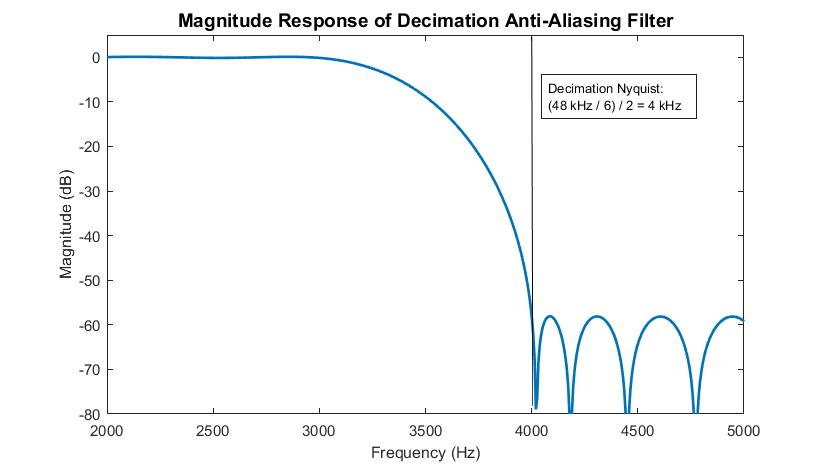
\includegraphics[width=0.8\textwidth]{./MagResp}
\caption{Magnitude response of anti-aliasing filter}
\label{f:figa}
\end{figure}

Additionally, the low- and high-pass filters implemented in project three were recycled for project four. The filters had stop and pass bands at 350 Hz/1310 Hz and 2100 Hz/1400 Hz, respectively. And the filters had 125 and 124 coefficients, respectively.

\subsection{Program Description}

The program consisted of two HWI threads, two TSK threads, two IDL threads and two MBXs. Figure \ref{f:fig2} illustrates the overall flow of the program in a block diagram. Audio was sampled by the stereo in the ADC and the samples were managed by the I2S receive HWI. The HWI stored copies of the samples in two arrays: one for audio processing/playback and one for decimation/signal display. Once the necessary number of samples had been collected, the receive HWI posted the array of samples to one of two arrays which corresponded to a specific TSK. The MBXs eliminated the need to pass a global array and posting to the MBX was analagous to posting a SWI. Depending on which MBX was posted, the program could follow two routes.

\begin{figure}[h]
\centering
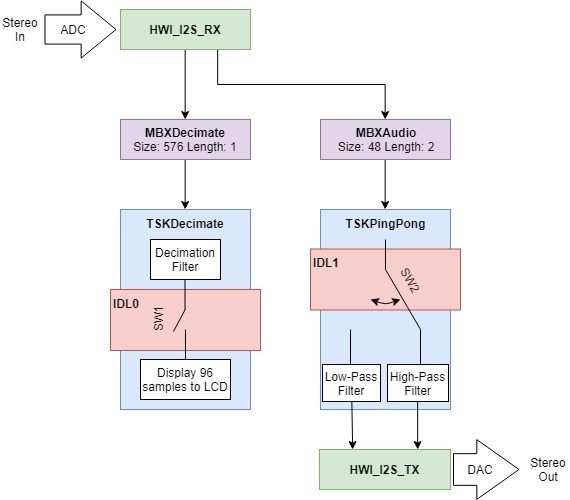
\includegraphics[width=0.8\textwidth]{./blocks}
\caption{Block diagram of program flow.}
\label{f:fig2}
\end{figure}

Similar to the ping-pong array used in project three, the MBX for the audio processing TSK had a length of two and a size of 48. In such a manner, the HWI could post 48 samples to the MBX and then continue storing new samples to be posted next. Until the HWI posted to the MBX, the audio processing TSK had been essentially waiting or pending on the HWI. After the MBX post, the TSK was no longer pending and began filtering audio using myfir, which stored values to a txPingPong array, similar to project three. The transmit HWI wrote filtered audio samples to the DAC to be played back to the listener. Again, an IDL thread was used to monitor for switch two presses and switched filter types in response.

The second MBX had a length of one and a size of 576. A total of 576 samples were collected before posting to this MBX because it was determined that 576 samples at 48 kHz were necessary to generate 96 samples after decimating by 6 (i.e. 96*6=576). Once the MBX was posted the second TSK stopped pending and began to run. However, it should be noted the audio processing TSK was given a higher priority such that the display TSK wouldn't interfere with the real-time requirement of the audio processing. The TSK took the 576 samples from the MBX and passed them through an anti-aliasing filtering using myfir. Again, when decimating, the sampling frequency is reduced by an integer factor and the Nyquist frequency is also reduced by the same factor. Therefore, all frequency components above the new Nyquist must be removed to avoid aliasing. After performing the filtering, decimation by a factor of six was performed by storing every sixth element of the 576 element array. The anti-aliasing and decimation was performed every time the receive HWI posted to the MBX, in order to have samples continually ready to be displayed.

An additional IDL thread was used to monitor switch one presses. When switch one was pressed, the IDL changed a global state variable that notified the display TSK that it should display an audio signal to the LCD. The LCD functions were taken from an example program provided by TI. To display the audio signal, the correct pixels had to be turned on according to the sample value. Only 16 pixels were available in each column; therefore, samples had to be binned according to their relative value. First, if the sample was positive it was placed in the top eight pixels of a column. Otherwise, it was placed in the bottom eight pixels. A value for the pixel was initially set near the center and a for loop was used to divide max value in either direction 32767 or 32768 into 8 bins. By looping through each area the value was checked against the new minimum absolute value for the bin. If the sample value was larger, then pixel value was bit shifted by one bit in such a manner that it was shifted away from the center. After determining the correct position in the column, the location was sent to the LCD chip and the send function advanced the display to the next column. Before sending the audio signal to the LCD, the display was cleared.

\section{Results}

\subsection{Display}

Using a GPIO pin, it was determined that it took the approximately 634 ms to clear and write to the display. Based on the fact that a frame is 96 samples, it was estimated that the frame rate was 1.6 frames per second. Ultimately, using the provided functions  introduced unneccessary tasks for sending pixels that inflated the time requirement. Also, a more efficient way of clearing the existing pixels would have eliminated a significant portion of the display time.

While many methods of improving frame rate may be applied, the rate is limited by the slow I2C communication line. A typical I2C operates at 100 kbits/s to 400 kbits/s. At 96 samples per frame, 16 bits per sample and a max transmission speed of 400 kbits/s, the maximum frame rate would be 260 frames per second. And if the I2C were limited to 100 kbits/s, then the maximum frame rate would be 65 frames per second. At 100 kbits/s, the current display method is operating at 2.5\% of peak efficiency. 

\subsection{Execution Graph}

Figure \ref{f:fig3} shows an execution graph with the I2S rx HWI (top), audio processing TSK (middle), and decimation/disply TSK (bottom). As expected, the audio processing TSK pends unitl 48 samples had been collected, runs, and pends until another 48 samples were  collected. Additionally, the execution graph shows decimation TSK running, but it does not show how long the TSK pends. It was expeceted that 576 rx HWI samples would have occured before the TSK quit pending again. Based on that assumption, it would have taken 12 milliseconds. 

Furthermore, the execution graph shows the time required by the audio processing TSK to process 48 samples: 142.5 microseconds. That means that the TSK is taking approximately 297 cycles per sample which is within the bounds of operating in real-time. Even the decimation filter is operating in real-time (392 cycles per sample). However, when the display component is introduced the TSK no longer operates in real-time (110462 cycles per sample).

\begin{figure}[h]
\centering
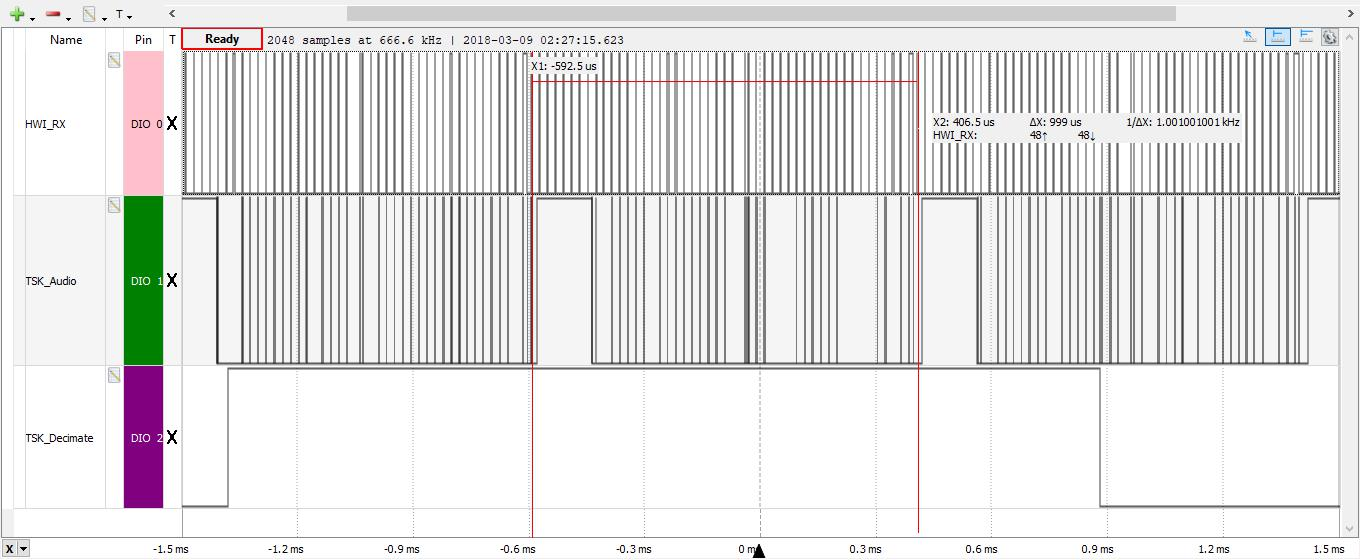
\includegraphics[width=0.8\textwidth]{./exec}
\caption{Execution of I2S rx HWI, ping-pong TSK, and decimation TSK }
\label{f:fig3}
\end{figure}

\subsection{Decimation}

Figure \ref{f:fig4} shows a discrete time plot of samples delivered to the decimation TSK before anti-aliasing, after anti-aliasing, and after decimation. The plot is not actually drawn to scale, it was plotted to illustrate that decimated samples align with every sixth sample provided by the anti-aliasing filter, which would be expected when decimating by six. Furthermore, if it were plotted to the actual number of the sample in the signal, then the decimated signal would appear as a compressed version of the original. When observing Figure \ref{f:fig5}, the decimated signal generated by the DSP board has a frequency that is expanded. Therefore, it makes sense that the time domain signal would compress because expansion in frequency is contraction in time and vice-versa. Furthermore, what is observed in Figure \ref{f:fig5} is that at higher sampling rates more frequency components are distributed across the Nyquist range. When the signal is decimated a small portion of the original Nyquist range is essentially expanded to cover the entire Nyquist range (speaking relatively and in terms of periodicity). Therefore, such an observation again shows that a successful decimation filter has been implemented. 

\begin{figure}[h]
\centering
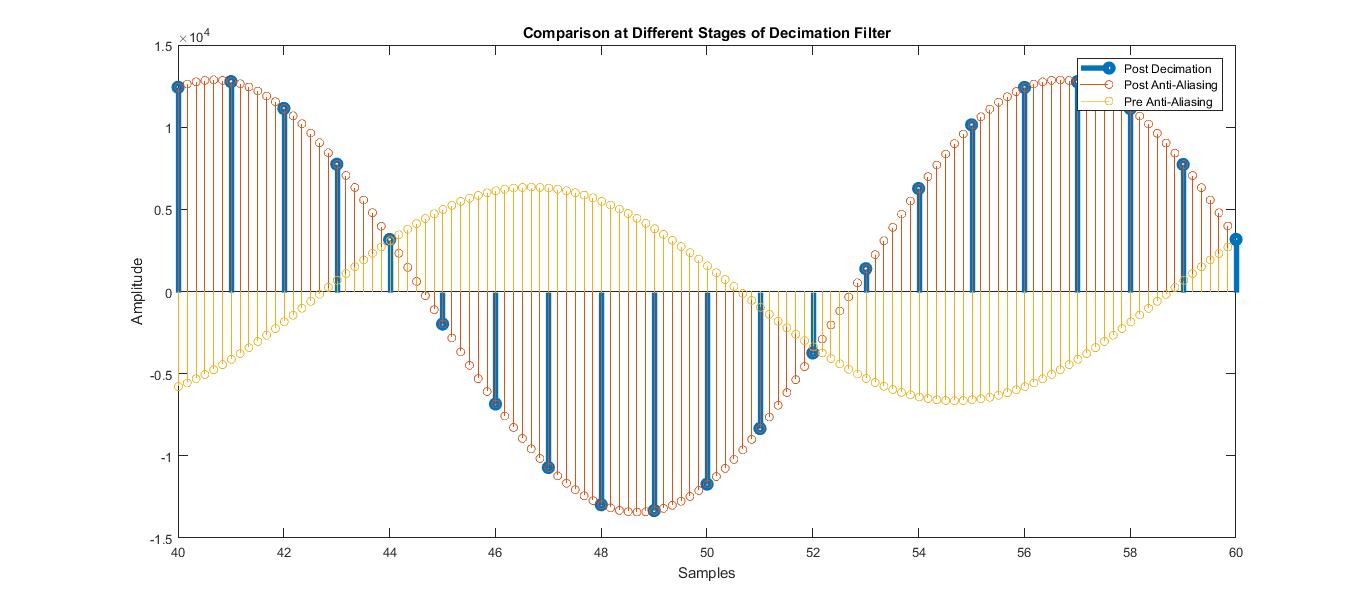
\includegraphics[width=0.8\textwidth]{./decimation}
\caption{A discrete time plot of data generated from the anti-aliasing filter and the decimation filter }
\label{f:fig4}
\end{figure}

\begin{figure}[h]
\centering
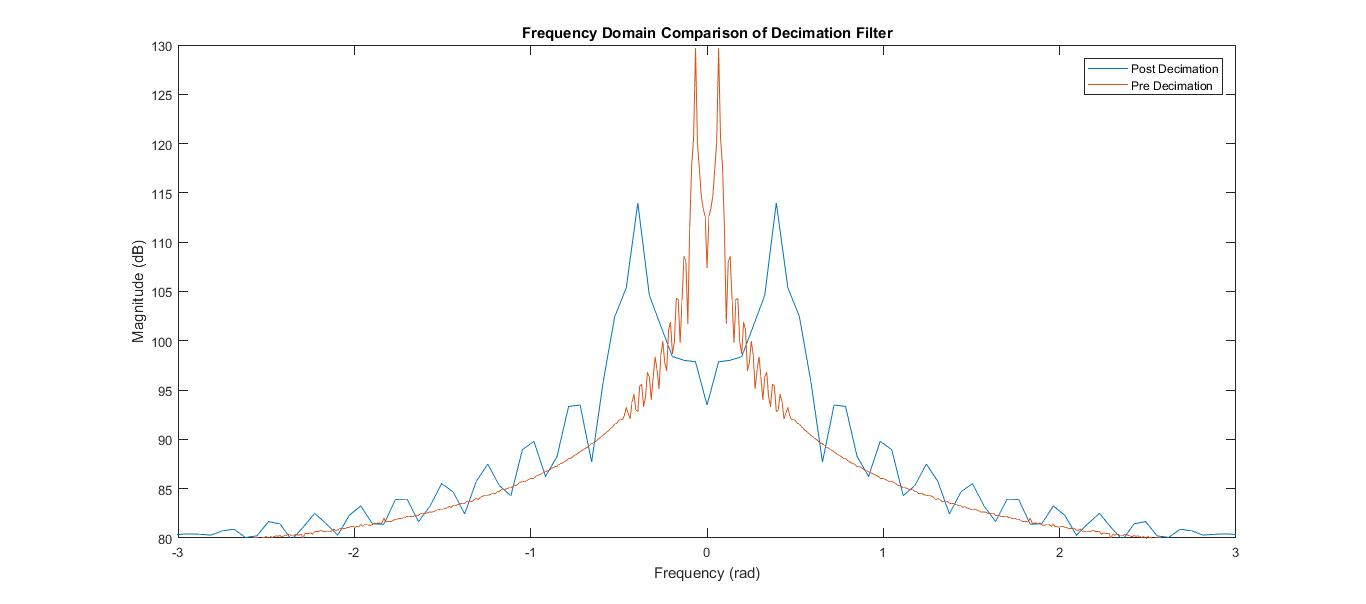
\includegraphics[width=0.8\textwidth]{./freqDec}
\caption{A frequency domain plot of data generated from the anti-aliasing filter and the decimation filter }
\label{f:fig5}
\end{figure}

\pagebreak

\section{Appendix}

\begin{lstlisting}[caption={main.c}, label=l:program1]
/*
 *  Copyright 2010 by Texas Instruments Incorporated.
 *  All rights reserved. Property of Texas Instruments Incorporated.
 *  Restricted rights to use, duplicate or disclose this code are
 *  granted through contract.
 *
 */
/***************************************************************************/
/*                                                                         */
/*     H E L L O . C                                                       */
/*                                                                         */
/*     Basic LOG event operation from main.                                */
/*                                                                         */
/***************************************************************************/

#include <std.h>

#include <log.h>

#include "hellocfg.h"
#include "ezdsp5535.h"
#include "ezdsp5535_i2s.h"
#include "ezdsp5535_lcd.h"
#include "ezdsp5535_led.h"
#include "ezdsp5535_sar.h"
#include "csl_i2s.h"
#include "stdint.h"
#include "aic3204.h"

extern CSL_I2sHandle   hI2s;
extern void audioProcessingInit(void);


void main(void)
{
    LOG_printf(&trace, "hello world!");

    /* Initialize BSL */
    EZDSP5535_init( );

    /* init LEDs and set to off*/
    EZDSP5535_LED_init( );
    EZDSP5535_LED_setall(0x0F);

    /* init dip switches */
    EZDSP5535_SAR_init( );

	/* Initialize OLED display */
    EZDSP5535_OSD9616_init( );
    EZDSP5535_OSD9616_send(0x00,0x2e);  // Deactivate Scrolling
    EZDSP5535_OSD9616_send(0x00,0x2e);  // Deactivate Scrolling

    // configure the Codec chip
    ConfigureAic3204();

    /* Initialize I2S */
    EZDSP5535_I2S_init();

    /* enable the interrupt with BIOS call */
    C55_enableInt(14); // reference technical manual, I2S2 tx interrupt
    C55_enableInt(15); // reference technical manual, I2S2 rx interrupt

    audioProcessingInit();

    // after main() exits the DSP/BIOS scheduler starts
}

\end{lstlisting}
\pagebreak

\begin{lstlisting}[caption={audioProcessing.c}, label=l:program2]
/*
 *  Copyright 2010 by Texas Instruments Incorporated.
 *  All rights reserved. Property of Texas Instruments Incorporated.
 *  Restricted rights to use, duplicate or disclose this code are
 *  granted through contract.
 *
 */
/***************************************************************************/
/*                                                                         */
/*     H E L L O . C                                                       */
/*                                                                         */
/*     Basic LOG event operation from main.                                */
/*                                                                         */
/***************************************************************************/

#include <std.h>

#include <log.h>

#include "stdint.h"
#include "string.h"
#include "hellocfg.h"
#include "ezdsp5535.h"
#include "ezdsp5535_gpio.h"
#include "ezdsp5535_i2s.h"
#include "ezdsp5535_led.h"
#include "ezdsp5535_sar.h"
#include "csl_i2s.h"
#include "csl_gpio.h"
#include "aic3204.h"
#include "filters.h"

#define NX			48
#define BL_ONLY		0x0E
#define YL_ONLY		0x0D
#define RD_ONLY		0x0B
#define GR_ONLY		0x07
#define MIN(a,b) ( ((a) <  (b)) ? (a) : (b) )

extern CSL_I2sHandle   hI2s;
extern void myfir(const int16_t* input, const int16_t* filterCoeffs,
		int16_t* output, int16_t* delayLine, uint16_t  nx, uint16_t  nh);
extern int16_t myNCO(uint16_t f_tone);
extern void clearPA(void);

int16_t rxPingPong[96];
int16_t txPingPong[96];
int16_t preDecSamps[576], preAA[576], postAA[576];
int16_t delayLineAA[576 + 121 - 1];
int16_t disp96[96];
int16_t finalDisp[96];

int16_t delayLineLPF[NX + LPF_NH - 1];
int16_t delayLineHPF[NX + HPF_NH - 1];

int16_t rxIndex;
int16_t txIndex;
int16_t ppIndex;
int16_t preDecIndex;
int16_t dispIndex;
int16_t deciIndex;

uint16_t sw1State  = 0;       	// SW1 state
uint16_t sw2State  = 0;       	// SW2 state
uint16_t filtState = 0;			// filter state

int16_t * filterPtr;
int16_t * delayLinePtr;
uint16_t myNH;


Uint16 idl = 0, swi = 0;

int displayGraph = 0;

extern void oscDisplay(int16_t * samples, int numSamps);

/*
 * audioProcessingInit
 *
 * @brief: 	Initialize arrays used for filtering and transmitting
 * 			and initialize array indices to 0.
 */
void audioProcessingInit(void)
{
	/* Initialize arrays as empty*/
	memset(txPingPong, 0, sizeof(txPingPong));
	memset(delayLineLPF, 0, sizeof(delayLineLPF));
	memset(delayLineHPF, 0, sizeof(delayLineHPF));

	/* Initially select low-pass filter */
	filterPtr = &myLPF[0];
	delayLinePtr = &delayLineLPF[0];
	myNH = LPF_NH;

	/* Initialize rx and tx indices to 0 */
	rxIndex = 0;
	txIndex = 0;
	ppIndex = 0;
	preDecIndex = 0;
	deciIndex = 0;
	dispIndex = 0;
}

/**********************************************************************
 *******************              HWIs              *******************
 **********************************************************************/

/*
 * HWI_I2S_Rx
 *
 * @brief: 	Function handle for HWI 15. Stores received samples into a
 * 			double buffer and post SWIs to perform filtering.
 */
void HWI_I2S_Rx(void)
{
//	EZDSP5535_GPIO_setOutput( 14, 1 );

	/* Read right sample and disregard. Read left sample and store
	 * in rxPingPong.
	 * Ping -> first 48 samples in array (0 - 47)
	 * Pong -> second 48 samples in array (48 - 97)
	 */
	volatile int16_t temp;
	temp = hI2s->hwRegs->I2SRXRT1;
	rxPingPong[rxIndex++] = hI2s->hwRegs->I2SRXLT1;
	preDecSamps[preDecIndex++] = temp;

	if (rxIndex == 48)		//Have 48 samples been collected
	{
		/* Ping is full -> Post SWIPing to run SWI that will
		 * filter the ping samples.
		 */
		MBX_post(&MBXAudio, &rxPingPong[0], 0);
	}

	if (rxIndex == 96)
	{
		/* Pong is full -> Post SWIPong to run SWI that will
		 * filter the pong samples. Clear rxIndex so rxPingPong
		 * will begin filling ping again.
		 */
		MBX_post(&MBXAudio, &rxPingPong[48], 0);
		rxIndex = 0;
	}

	if(preDecIndex == 576)
	{
		MBX_post(&MBXDecimate, &preDecSamps[0], 0);
		preDecIndex = 0;
	}

	EZDSP5535_GPIO_setOutput( 14, 0 );
}

/*
 * HWI_I2S_Tx
 *
 * @brief: 	Function handle for HWI 14. Transmits filtered samples
 * 			from a double buffer.
 */
void HWI_I2S_Tx(void)
{
	/* Transmit filtered samples */
	hI2s->hwRegs->I2STXLT1 = txPingPong[txIndex];
	hI2s->hwRegs->I2STXRT1 = txPingPong[txIndex++];

	if (txIndex == 96)		//Have 96 samples been transmitted?
	{
		/* Set index to beginning of tx array */
		txIndex = 0;
	}
}

/**********************************************************************
 *******************              TSKs              *******************
 **********************************************************************/

void TSKPingPongFunc(void)
{
	int16_t ping[48], pong[48];

    /* Filter a frame of 48 received samples and store output in tx buffer
     *  using myfir. Variables filterPtr and delayLinePtr point to the desired
     *  filter (LPF or HPF) and it's corresponding delayline (selected in second IDL
     *  thread).
     */
	while(1)
 	{
		if(ppIndex == 0)
		{
	 		MBX_pend(&MBXAudio, &ping, SYS_FOREVER);
//			EZDSP5535_GPIO_setOutput( 15, 1 );
	 		myfir(&ping[0], filterPtr, &txPingPong[0], delayLinePtr, NX, myNH);
	 		ppIndex = 1;
		} else if (ppIndex == 1)
		{
	 		MBX_pend(&MBXAudio, &pong, SYS_FOREVER);
//			EZDSP5535_GPIO_setOutput( 15, 1 );
	 		myfir(&pong[0], filterPtr, &txPingPong[48], delayLinePtr, NX, myNH);
	 		ppIndex = 0;
		}

//		EZDSP5535_GPIO_setOutput( 15, 0 );
 	}
}

void TSKDecimateFunc(void)
{
	int i;

	while(1)
	{
		MBX_pend(&MBXDecimate, &preAA, SYS_FOREVER);
//		EZDSP5535_GPIO_setOutput( 17, 1 );
		myfir(&preAA[0], sharpAA, &postAA[0], delayLineAA, 576, 121);
		IDL_run();

		disp96[0] = postAA[0];

		for(i = 6; i < 576; i++)
		{
			if((i % 6) == 0)
			{
				disp96[i/6] = postAA[i];
			}
		}

		IDL_run();
		if(displayGraph == 1)
		{
			oscDisplay(disp96, 96);
			displayGraph = 0;
		}

//		EZDSP5535_GPIO_setOutput( 17, 0 );
	}
}

/**********************************************************************
 *******************              IDLs              *******************
 **********************************************************************/

void monitorSW1(void)
{
	/* Check SW1 */
	if(EZDSP5535_SAR_getKey( ) == SW1) 		// Is SW1 pressed?
	{
		if(sw1State)             			// Was previous state not pressed?
		{
			displayGraph = 1;				//Tell TSK to display graph

			sw1State = 0;     				// Set state to 0 to allow only single press
		}
	} else                      			// SW1 not pressed
	{
		sw1State = 1;         				// Set state to 1 to allow timer change
	}
}

void monitorSW2(void)
{
	/* Check SW2 */
	if(EZDSP5535_SAR_getKey( ) == SW2) 		// Is SW2 pressed?
	{
		if(sw2State)          				// Was previous state not pressed?
		{
			if(filtState)					//Was previous state High-pass?
			{
				/* Clear Low-pass delayLine */
				memset(delayLineLPF, 0, sizeof(delayLineLPF));

				/* Point filter pointer to myLPF */
				filterPtr = &myLPF[0];

				/* Point delay line pointer to delayLineLPF */
				delayLinePtr = &delayLineLPF[0];

				/* Set myNH to number of low-pass coefficients */
				myNH = LPF_NH;

				/* Set filtState to low-pass */
				filtState = 0;
			} else				//Was previous state low-pass
			{
				/* Clear high-pass delay line */
				memset(delayLineHPF, 0, sizeof(delayLineHPF));

				/* Point filter pointer to myHPF */
				filterPtr = &myHPF[0];

				/* Point delayline pointer to delayLineHPF */
				delayLinePtr = &delayLineHPF[0];

				/* Set my NH to number of high-pass coefficients */
				myNH = HPF_NH;

				/* Set filtState to high-pass */
				filtState = 1;
			}
			sw2State = 0;     				// Set state to 0 to allow only single press
		}
	} else                      			// SW2 not pressed
	{
		sw2State = 1;         				// Set state to 1 to allow tone change
	}
}
\end{lstlisting}
\pagebreak

\begin{lstlisting}[caption={oscDisplay.c}, label=l:program3]
/*
 * oscDisplay.c
 *
 *  Created on: Mar 8, 2018
 *      Author: Zach
 */

#include "stdint.h"
#include "ezdsp5535_lcd.h"
#include "ezdsp5535_gpio.h"

void pixLoc(int16_t sample, int * topBot, Uint16 * loc8)
{
	int i;

	if(sample < 0 )
	{
		*loc8 = 0x01;
		* topBot = 1;
		sample = sample * (-1);

		for( i = 1; i < 8; i++)
		{
			if(sample > (i * (32768 / 8)))
			{
				* loc8 = (* loc8) << 1;
			}
		}
	} else if(sample > 0) {
		*loc8 = 0x80;
		* topBot = 0;

		for( i = 1; i < 8; i++)
		{
			if(sample > (i * (32768 / 8)))
			{
				* loc8 = (* loc8) >> 1;
			}
		}
	} else {
		*loc8 = 0x00;
		*topBot = 0;
	}
}

void oscDisplay(int16_t * samples, int numSamps)
{
//	Uns olstate = HWI_disable();
//	TSK_disable();

//	EZDSP5535_GPIO_setOutput( 14, 0 );

	int i, j;
	int topBot;
	Uint16 loc8;

	/* Fill page 0 */
	EZDSP5535_OSD9616_send(0x00,0x00);   // Set low column address
	EZDSP5535_OSD9616_send(0x00,0x10);   // Set high column address
	EZDSP5535_OSD9616_send(0x00,0xb0+0); // Set page for page 0 to page 5

	for(i=0;i<128;i++)
	{
		EZDSP5535_OSD9616_send(0x40,0x00);
	}

	/* Fill page 1*/
	EZDSP5535_OSD9616_send(0x00,0x00);   // Set low column address
	EZDSP5535_OSD9616_send(0x00,0x10);   // Set high column address
	EZDSP5535_OSD9616_send(0x00,0xb0+1); // Set page for page 0 to page 5

	for(i=0;i<128;i++)
	{
		EZDSP5535_OSD9616_send(0x40,0x00);
	}

	EZDSP5535_OSD9616_send(0x00,0x00);   // Set low column address
	EZDSP5535_OSD9616_send(0x00,0x10);   // Set high column address

	for(j = 0; j < 96; j++)
	{
		pixLoc(samples[j], &topBot, &loc8);
		EZDSP5535_OSD9616_send(0x00,0xb0+topBot); // Set page for page 0 to page 5
		EZDSP5535_OSD9616_send(0x40,loc8);
	}

//	EZDSP5535_GPIO_setOutput( 14, 1 );

//	HWI_restore(olstate);
//	TSK_enable();
}
\end{lstlisting}
\pagebreak

\begin{lstlisting}[caption={filters.h}, label=l:program4]
/*******************************************************************************
****                         D E F I N I T I O N S
*******************************************************************************/
#define LPF_NH		126
#define HPF_NH		125
/*******************************************************************************
****                    G L O B A L   V A R I A B L E S
*******************************************************************************/

int16_t myLPF[] =
{
       -23,    -13,    -16,    -20,    -24,    -28,    -33,    -38,    -43,    -49,    -55,    -60,    -66,    -72,    -77,    -82,
       -86,    -90,    -93,    -95,    -96,    -95,    -93,    -89,    -84,    -77,    -68,    -56,    -42,    -26,     -8,     13,
        36,     62,     90,    121,    154,    189,    226,    265,    306,    348,    391,    435,    480,    525,    571,    615,
       660,    703,    745,    785,    823,    859,    892,    922,    950,    973,    993,   1010,   1022,   1030,   1034,   1034,
      1030,   1022,   1010,    993,    973,    950,    922,    892,    859,    823,    785,    745,    703,    660,    615,    571,
       525,    480,    435,    391,    348,    306,    265,    226,    189,    154,    121,     90,     62,     36,     13,     -8,
       -26,    -42,    -56,    -68,    -77,    -84,    -89,    -93,    -95,    -96,    -95,    -93,    -90,    -86,    -82,    -77,
       -72,    -66,    -60,    -55,    -49,    -43,    -38,    -33,    -28,    -24,    -20,    -16,    -13,    -23
};

int16_t myHPF[] =
{
       -24,   -147,      6,    -15,     -6,      1,     10,     20,     31,     43,     53,     62,     69,     73,     73,     69,
        60,     46,     27,      5,    -21,    -49,    -78,   -106,   -132,   -153,   -169,   -177,   -176,   -166,   -144,   -113,
       -71,    -20,     38,    102,    168,    233,    294,    347,    388,    414,    420,    405,    366,    300,    209,     91,
       -53,   -219,   -404,   -605,   -817,  -1034,  -1251,  -1460,  -1657,  -1835,  -1989,  -2115,  -2207,  -2263,  30486,  -2263,
     -2207,  -2115,  -1989,  -1835,  -1657,  -1460,  -1251,  -1034,   -817,   -605,   -404,   -219,    -53,     91,    209,    300,
       366,    405,    420,    414,    388,    347,    294,    233,    168,    102,     38,    -20,    -71,   -113,   -144,   -166,
      -176,   -177,   -169,   -153,   -132,   -106,    -78,    -49,    -21,      5,     27,     46,     60,     69,     73,     73,
        69,     62,     53,     43,     31,     20,     10,      1,     -6,    -15,      6,   -147,    -24
};

/* Anti-aliasing filter for decimation Fpass = 3 kHz 0.2 dB, Fstop = 4 kHz -60 dB */
int16_t sharpAA[] =
{
        19,     -5,    -13,    -25,    -39,    -53,    -64,    -67,    -62,    -47,    -22,      8,     40,     67,     83,     84,
        67,     33,    -13,    -62,   -105,   -132,   -135,   -110,    -58,     13,     91,    159,    203,    210,    174,     95,
       -13,   -133,   -241,   -312,   -326,   -273,   -155,     12,    201,    375,    494,    525,    449,    263,    -12,   -334,
      -646,   -880,   -972,   -868,   -540,     11,    753,   1621,   2527,   3374,   4063,   4513,   4670,   4513,   4063,   3374,
      2527,   1621,    753,     11,   -540,   -868,   -972,   -880,   -646,   -334,    -12,    263,    449,    525,    494,    375,
       201,     12,   -155,   -273,   -326,   -312,   -241,   -133,    -13,     95,    174,    210,    203,    159,     91,     13,
       -58,   -110,   -135,   -132,   -105,    -62,    -13,     33,     67,     84,     83,     67,     40,      8,    -22,    -47,
       -62,    -67,    -64,    -53,    -39,    -25,    -13,     -5,     19
};

\end{lstlisting}
\pagebreak

\begin{lstlisting}[caption={myfir.c}, label=l:program5]
/*
// *****************************************************************************
// *****************************************************************************
// **
// ** File Name: myfir.c
// **
// ** Author: David McCreight
// **
// ** Description: 
// **              
// **
// *****************************************************************************
// *****************************************************************************
*/

/*******************************************************************************
****                            I N C L U D E S 
*******************************************************************************/

#include "stdint.h"
#include "stdio.h"

/*******************************************************************************
****                         D E F I N I T I O N S
*******************************************************************************/

/*******************************************************************************
****                   S T A T I C   V A R I A B L E S  
*******************************************************************************/

/*******************************************************************************
****                    G L O B A L   V A R I A B L E S  
*******************************************************************************/

/*******************************************************************************
****          F U N C T I O N   D E F I N I T I O N S 
*******************************************************************************/
void myfir(const int16_t* input,
             const int16_t* filterCoeffs,
			 int16_t* output,
			 int16_t* delayLine,
			 uint16_t  nx,
			 uint16_t  nh)
{
    
    uint16_t i;
    uint16_t j;
    long sum = 0;
	
    /*
     * Assumes delayLine length is nh - 1 + nx
     */

    // copy input samples to the delay line
    for (i = 0; i < nx; i++)
    {
        delayLine[i + nh - 1] = input[i];
    }

	for (i = 0; i < nx; i++)
	{
		for (j = 0; j < nh; j++)
		{
			sum = _smacr(sum, filterCoeffs[j], delayLine[i + nh - 1 - j]);
		}

		output[i] = (int16_t)(sum >> 15);
		sum = 0;
	}
		
    // Update delay line for next function call
	for (i = 0; i < (nh - 1); i++)
	{
		delayLine[i] = delayLine[nx + i];
	}
}

/*******************************************************************************
 ****                        E N D   O F   F I L E
 *******************************************************************************/
\end{lstlisting}
\end{document}



